\apendice{Especificación de diseño}

\section{Introducción}

	En este apartado del trabajo se van a marcar varios aspectos importantes como la forma de guardar los datos en la base de datos, los diagramas de casos de uso o la conexión de los distintos elementos, entre otras cosas.

\section{Diseño de datos}

	Como se ha indicado en otros puntos de este trabajo, la base de datos utilizada ha sido Firestore Database. Esta base de datos, albergada en la nube y propiedad de Google, responde a la filosofía NoSQL. Para situarnos, una vez que entramos en la base de datos nos encontramos la ventana representada en la Figura \ref{fig:db1}.
	
\imagen{db1}{Pantalla principal Firestore Database}

	Esta base de datos denomina las tablas con el nombre ``colecciones'', mientras que los registros de cada una de ellas reciben el nombre de ``documentos''. Si queremos ingresar los datos de manera manual, simplemente debemos seguir lo siguientes pasos:
	\begin{enumerate}
		\item Situarnos en la colección donde queramos guardar un nuevo registro.
		\item Pulsar en el botón de la columna central ``+ Agregar documento''
		\item En la ventana modal, establecer un identificador único a cada ``documento'' (suelen generarse de manera automática) y completar añadiendo los campos que se deseen siguiendo: campo-tipo-valor
	\end{enumerate}
	
	En relación a este trabajo, se han necesitado tres colecciones: usuarios, relojes y subastas. A continuación se presentan la Figura \ref{fig:db3}, la Figura \ref{fig:db4} y la Figura \ref{fig:db2} que marcan los tipos de datos de cada colección respectivamente.
	
\imagen{db3}{Forma datos usuarios}
\imagen{db4}{Forma datos relojes}	
\imagen{db2}{Forma datos subasta}

	Sin embargo, los datos no se guardan de manera manual. Desde Flutter se han creado dos funciones capaces de enviar y recibir los datos entre ambas partes. Como ejemplo, la Figura \ref{fig:db5} y la Figura \ref{fig:db6} representan el código necesario para entablar tal comunicación con la colección \emph{auctions}.
	
\imagen{db5}{Conexión con Flutter parte 1}	
\imagen{db6}{Conexión con Flutter parte 2}

	La primera parte define el constructor para poder crear instancias de subastas, especificando dentro de ella tanto los campos que debe albergar como si son obligatorios de completar. Por otro lado, el método \emph{fromFirestore} es el método que crea una instancia a partir del documento que recibe de la base de datos en la nube.
	
	Si se quisiera realizar el sentido contrario, se utilizaría la función \emph{toMap}, la cual recoge una instancia y la convierte en un mapa. El porqué de esta conversión es que es el formato requerido para almacenar datos en Firestore Database.
	

\section{Diseño procedimental}

	No hay mejor forma de presentar el diseño procedimental que esquematizando el diagrama de casos de uso que pueden darse a lo largo del uso de la aplicación junto con sus digramas de secuencia. A continuación, de la Figura \ref{fig:casoUso1} hasta la Figura \ref{fig:casoUso13} (ambas incluidas) presentarán todo esto.
	
\imagen{casoUso1}{Iniciar sesión}
\imagen{casoUso2}{Registrar usuario}
\imagen{casoUso3}{Ver relojes}
\imagen{casoUso4}{Añadir reloj}
\imagen{casoUso5}{Editar reloj}
\imagen{casoUso6}{Eliminar reloj}
\imagen{casoUso7}{Ver subastas}
\imagen{casoUso8}{Crear subasta}
\imagen{casoUso9}{Eliminar subasta}
\imagen{casoUso10}{Pujar en una subasta}
\imagen{casoUso11}{Comprar reloj directamente en una subasta}
\imagen{casoUso12}{Editar información personal}
\imagen{casoUso13}{Consultar precio reloj}


\section{Diseño arquitectónico}

	Siguiendo un poco lo marcado en la introducción, es importante definir cómo se comunican las distintas partes de este trabajo. En el informe referente a la memoria se establecía que el patrón ``Modelo-Vista-Controlador'' o MVC iba a ser quien marcara la arquitectura dentro del proyecto Flutter. Sin embargo, también se debe tener en cuenta cómo se ha conectado la API del modelo de predicción de precios y la base de datos explicada anteriormente.
	Para ser más preciso, se presenta a través de la Figura \ref{fig:disenoArquitectonico} la conexión entre las distintas partes. Para ello, se va a seguir el proceso de una acción como ejemplo.

\imagen{disenoArquitectonico}{Esquema conexión de elementos}

	\begin{enumerate}
		\item Un usuario completa los campos del registro de un reloj y pulsa en el botón ``Añadir reloj''. La vista (en nuestro caso el \emph{widget}) se lo comunica al controlador (definido en el mismo \emph{script} que la vista).
		\item El controlador recoge la orden y se la envía al modelo.
		\item El modelo se comunica con la base de datos para realizar la orden de añadir el reloj.
		\item Si todo correcto, la base de datos realizará la acción sin problema.
		\item El modelo comunica al controlador que la acción se realizó correctamente.
		\item El controlador procesa esa información y se la comunica a la vista de la manera que sea pertinente.
		\item La vista muestra un mensaje de información asegurando la inserción del nuevo reloj.
		\item En el caso que se quisiera predecir el precio del reloj a la hora de añadir el reloj, es el controlador quien envía la orden directa a la API alojada en Render.
		\item Render devuelve la respuesta a esa consulta y es el controlador quien se lo comunica a la vista para que se muestre una ventana informativa con el resultado de la predicción.
	\end{enumerate}

\section{Diseño visual}

	Siempre es bueno realizar un pequeño esquema de cómo podrían verse las distintas pantallas de nuestra aplicación. Si es cierto que son bocetos que pueden distar bastante de la realidad, pero es una buena práctica si los realizamos en conjunto con el cliente. Al final lo que buscamos es entendernos con él lo mejor posible y que mejor que a través de un dibujo.
	
	En mi caso, decidí intentar representar las interfaces basándome en todos los requisitos explicados en apartados anteriores. Para ello, utilicé el sitio web NinjaMock, el cual ya había utilizado en anteriores asignaturas del grado.
	
	NinjaMock es una herramienta muy amigable y eficaz si nuestro objetivo es realizar bocetos de cómo podría quedar el \emph{front-end} de nuestra aplicación. Aunque tiene una versión de pago, este software nos brinda la oportunidad de crear un único proyecto con todas nuestras interfaces de manera gratuita.
	
	A continuación, adjuntamos las distintas interfaces haciendo breves comentarios de ellas donde fuera necesario.
	
\begin{figure}[H]
    \centering
    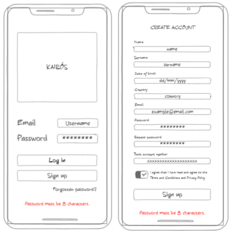
\includegraphics[width=0.6\linewidth]{img/image1.png}
    \caption{Diseño inicio de sesión y registro de cuenta}
    \label{fig:image1}
\end{figure}

	Como se puede apreciar en la Figura \ref{fig:image1}, en muchas de las ventanas lanzaremos mensajes a modo de advertencia al usuario si este no completa correctamente los campos requeridos. Todas las condiciones de cada campo se marcan en los requisitos expuestos.
	
\begin{figure}[H]
    \centering
    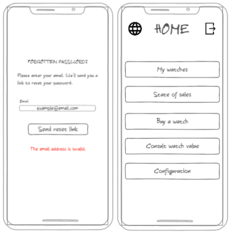
\includegraphics[width=0.6\linewidth]{img/image2.png}
    \caption{Diseño recuperación de contraseña y página principal}
    \label{fig:image2}
\end{figure}
	
	Según lo representado en la Figura \ref{fig:image2}, la idea de la recuperación de contraseña es reactivarla a través de un código al correo electrónico del usuario (aunque esto son líneas futuras). La mayoría de los iconos que nos llevan a alguna interfaz es porque se han marcado como iconos a ventanas emergentes para ayudar más al usuario.
	
\begin{figure}[H]
    \centering
    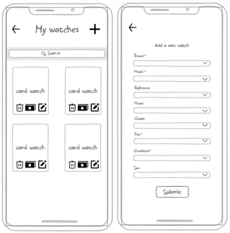
\includegraphics[width=0.6\linewidth]{img/image3.png}
    \caption{Diseño ver mis relojes y añadir nuevos}
    \label{fig:image3}
\end{figure}
	
	Según la Figura \ref{fig:image3}, los iconos son bastante explícitos. Destaco lo que se marca como un billete: será la puerta a la puesta en venta del reloj. Lo vemos en la Figura \ref{fig:image4} como ``creación de subasta''.
	
\begin{figure}[H]
    \centering
    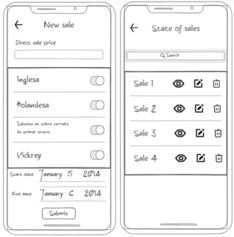
\includegraphics[width=0.6\linewidth]{img/image4.png}
    \caption{Diseño creación de subasta y estado de ventas}
    \label{fig:image4}
\end{figure}

\begin{figure}[H]
    \centering
    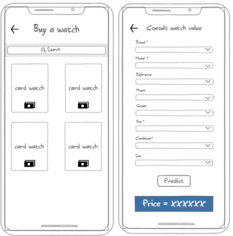
\includegraphics[width=0.6\linewidth]{img/image5.png}
    \caption{Diseño de aplicar a una subasta y predicción de precio}
    \label{fig:image5}
\end{figure}

	Al igual que en otras interfaces, el usuario podrá aplicar a la subasta directamente desde el botón representado en la Figura \ref{fig:image5}. Saldrá una ventana emergente donde marcará el precio a aplicar.
	
\begin{figure}[H]
    \centering
    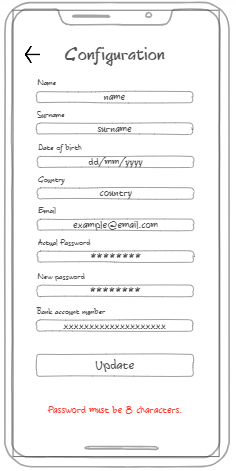
\includegraphics[width=0.6\linewidth]{img/image6.png}
    \caption{Diseño configuración de información personal}
    \label{fig:image6}
\end{figure}

	Hay que destacar sobre lo representado en la Figura \ref{fig:image6} que no debe cumplimentar todos los campos para configurar la información personal. Aun así, habrá campos que dependan unos de otros como los de contraseña.
